\section*{\color{red}III. Software Requirement Specification}

\subsection*{1. Product Overview}

Hệ thống Cá nhân hóa lộ trình học và Luyện thi Đánh giá năng lực tích hợp AI là một nền tảng giáo dục trên nền web (web-based) toàn diện. Hệ thống được thiết kế nhằm số hóa và tối ưu hóa quá trình ôn luyện, hỗ trợ đánh giá dựa trên năng lực chuẩn và tích hợp sâu các công nghệ AI tiên tiến (LLM + RAG) để đồng hành cùng Học sinh, Giáo viên, Phụ huynh và Quản trị viên trong suốt quá trình học tập.

Đoạn sơ đồ ngữ cảnh dưới đây thể hiện các tác nhân bên ngoài và giao diện tương tác với hệ thống:

\begin{figure}[h!]
	\centering
	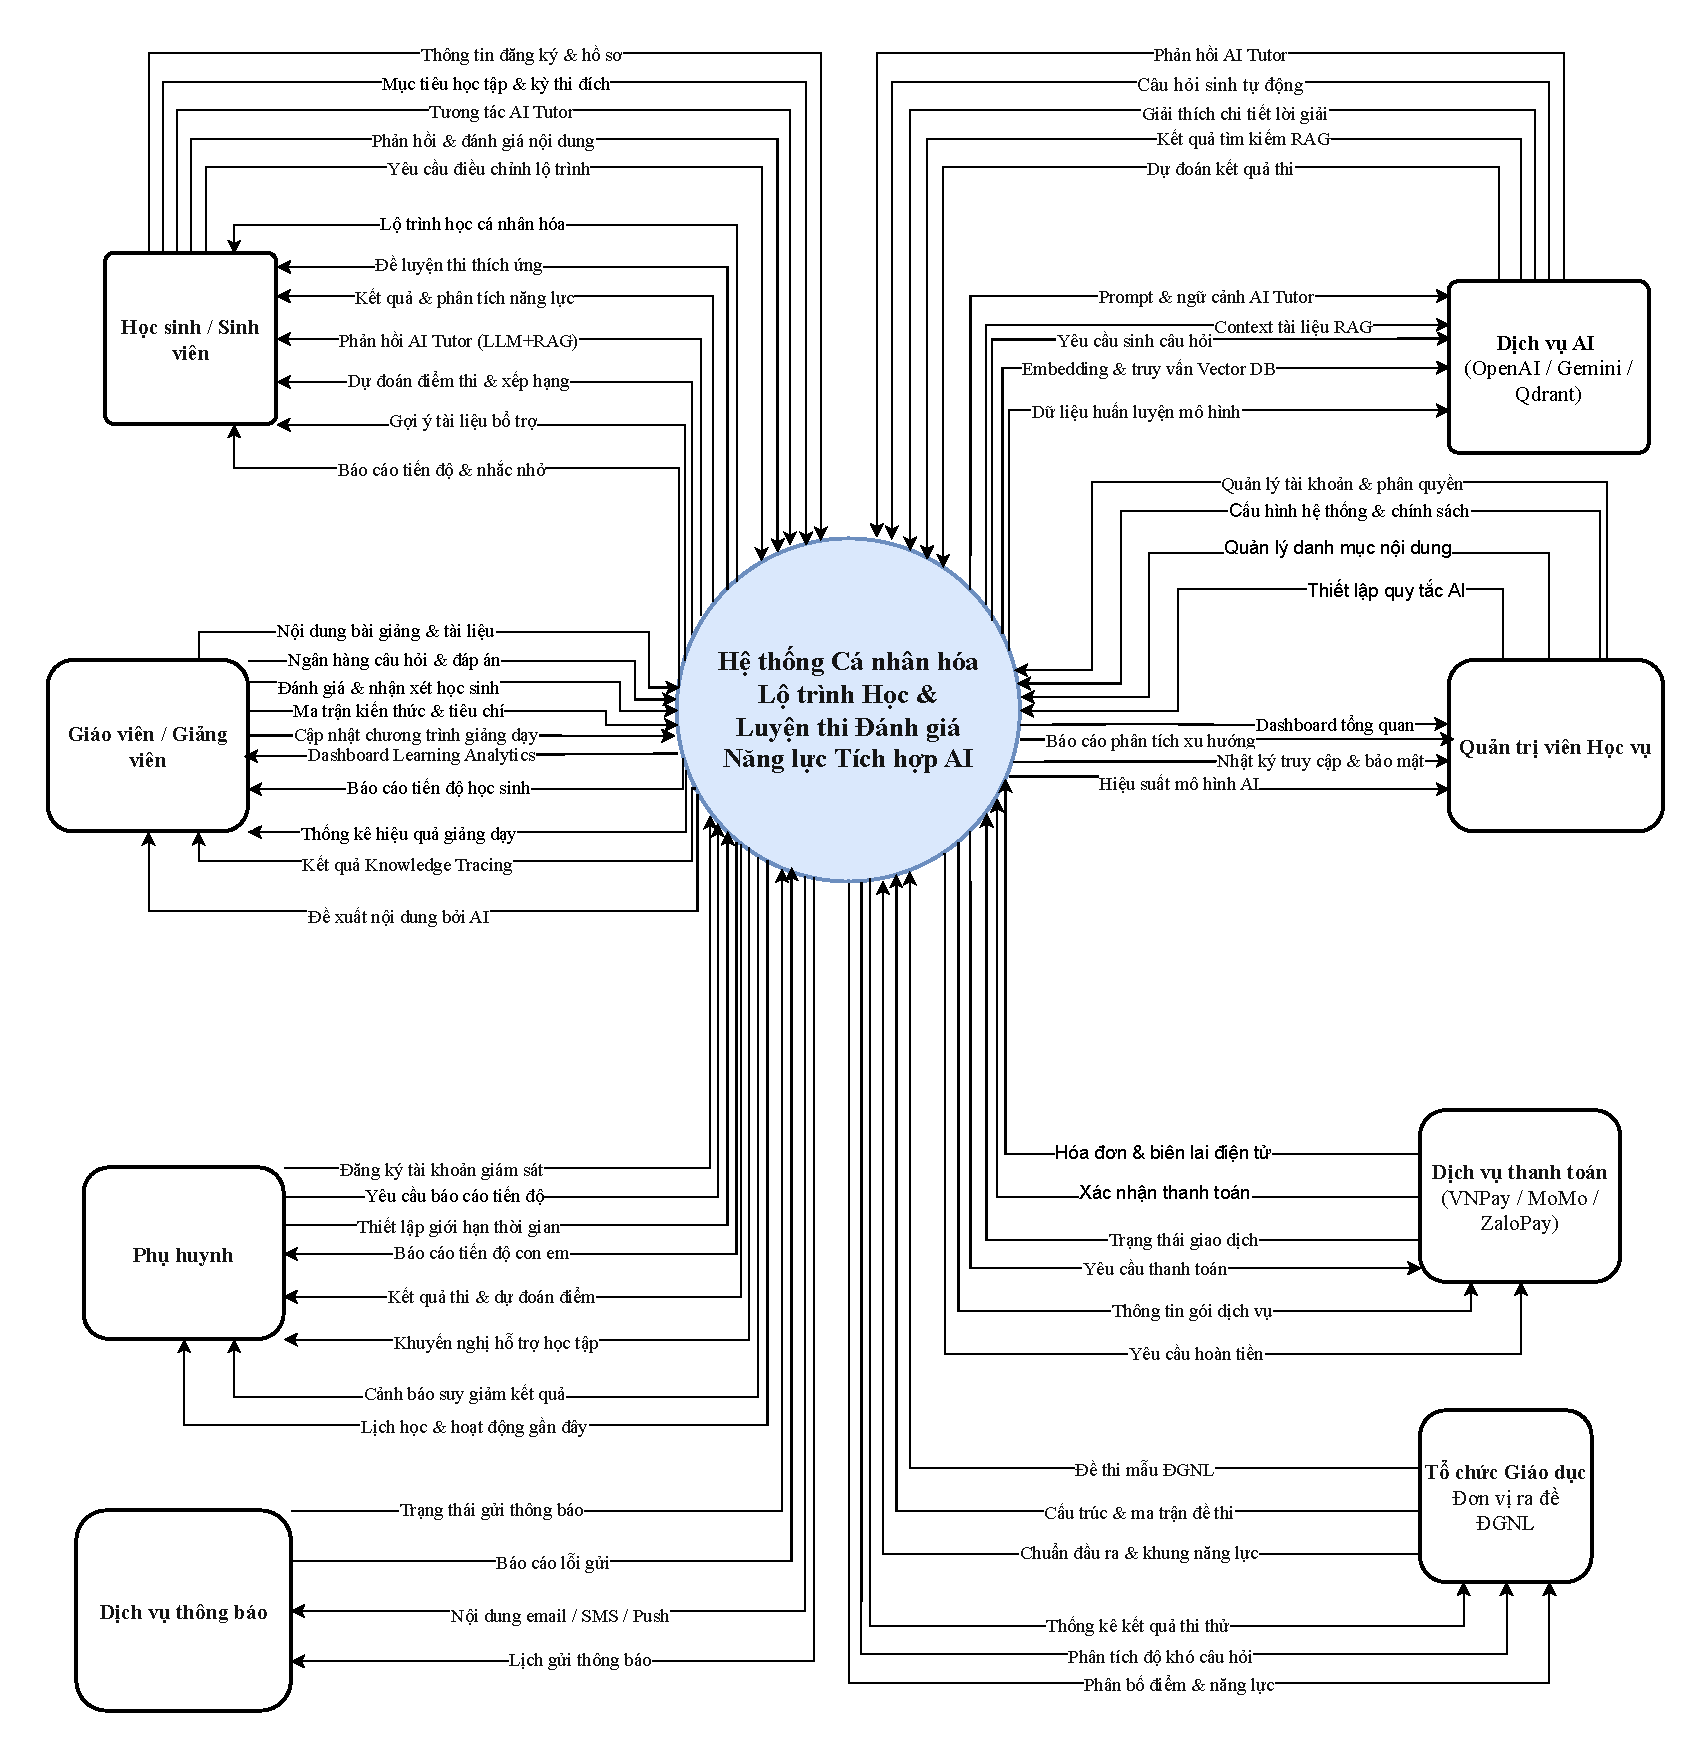
\includegraphics[width=0.9\textwidth]{Context_Diagram.pdf}
	\caption{Sơ đồ ngữ cảnh hệ thống (Context Diagram)}
	\label{fig:context_diagram}
\end{figure}

\begin{itemize}
	\item \textbf{Môi trường hoạt động (Operational Environment):}
	\begin{itemize}
		\item \textbf{Nền tảng (Platform):} Ứng dụng Web-based đa nền tảng, truy cập mượt mà qua các trình duyệt web hiện đại (Chrome, Edge, Firefox, Safari).
		\item \textbf{Kết nối (Connectivity):} Yêu cầu kết nối Internet liên tục và ổn định (không hỗ trợ chế độ offline) để xử lý các luồng dữ liệu đánh giá và truy vấn AI theo thời gian thực.
		\item \textbf{Hạ tầng (Infrastructure):} Triển khai trên nền tảng điện toán đám mây (Cloud-based) với kiến trúc linh hoạt, hỗ trợ tốt các API dịch vụ AI, Cơ sở dữ liệu Vector (Vector Database) và hệ thống Gateway gửi thông báo.
	\end{itemize}
	
	\item \textbf{Người dùng dự kiến (Anticipated Users):}
	\begin{itemize}
		\item \textbf{Người dùng nội bộ (Internal Users):} Quản trị viên Học vụ (Academic Administrator), Giáo viên / Giảng viên chuyên môn (Teacher / Lecturer).
		\item \textbf{Người dùng bên ngoài (External Users):} Học sinh / Sinh viên (Khách hàng chính), Phụ huynh (Parent).
		\item \textbf{Tác nhân hệ thống ngoài (External Systems):} Các dịch vụ API AI, Cổng thanh toán, Tổ chức Giáo dục.
	\end{itemize}
	
	\item \textbf{Ràng buộc \& Giả định (Constraints \& Assumptions):}
	\begin{itemize}
		\item Hệ thống bám sát phương pháp học tập và xây dựng lộ trình cá nhân hóa dựa trên chuẩn năng lực cốt lõi (competency-based).
		\item Các phân tích và đề xuất từ AI chỉ đóng vai trò như một ``Tutor'' hỗ trợ (Learning Assistance), tuyệt đối không thay thế các quyết định mang tính chuyên môn, học thuật của Giáo viên.
		\item Độ chính xác của kết quả đánh giá phụ thuộc chặt chẽ vào chất lượng ngân hàng câu hỏi và khung năng lực do các Tổ chức giáo dục đối tác cung cấp.
		\item Mọi giao dịch thanh toán trực tuyến phải được mã hóa và xử lý thông qua các cổng thanh toán nội địa uy tín.
	\end{itemize}
	
	\item \textbf{Tích hợp (Integrations):}
	\begin{itemize}
		\item Dịch vụ Trí tuệ nhân tạo (OpenAI / Gemini API).
		\item Cơ sở dữ liệu Vector chuyên dụng (Qdrant / Pinecone).
		\item Cổng thanh toán điện tử (VNPay / MoMo / ZaloPay).
		\item Dịch vụ truyền thông đa kênh (Email / SMS / Push Notification).
		\item Hệ thống dữ liệu của các Tổ chức Giáo dục cung cấp đề thi ĐGNL.
	\end{itemize}
	
	\item \textbf{Phụ thuộc (Dependencies):}
	\begin{itemize}
		\item Sự ổn định, tốc độ phản hồi (latency) và giới hạn tải (rate limits) của các API dịch vụ AI.
		\item Độ trễ và băng thông của Cơ sở dữ liệu Vector khi thực hiện tìm kiếm ngữ nghĩa (Semantic Search).
		\item Tính sẵn sàng của các API Cổng thanh toán và Dịch vụ Thông báo.
	\end{itemize}
\end{itemize}

\newpage

\subsection*{2. User Requirements}

\subsubsection*{2.1 Actors}

\begin{table}[h!]
	\centering
	\renewcommand{\arraystretch}{1.3}
	\begin{tabular}{|c|p{4cm}|p{9.5cm}|}
		\hline
		\rowcolor[HTML]{FCE4D6} 
		\textbf{\#} & \textbf{Tác nhân (Actor)} & \textbf{Mô tả vai trò \& Nhiệm vụ cốt lõi} \\ \hline
		
		1 & \textbf{Quản trị viên Học vụ} \newline (Academic Admin) & Chịu trách nhiệm vận hành toàn diện hệ thống: quản lý tài khoản, phân quyền truy cập (RBAC), quản lý nội dung học tập và thiết lập khung năng lực. Thực hiện cấu hình các chính sách và siêu tham số (hyperparameters) cho thuật toán AI. Giám sát luồng đồng bộ dữ liệu, theo dõi logs hoạt động và đánh giá hiệu suất tổng thể qua các bảng điều khiển (Dashboards) để xử lý sự cố. \\ \hline
		
		2 & \textbf{Giáo viên / Giảng viên} \newline (Teacher) & Đóng vai trò chuyên gia học thuật. Trực tiếp tạo lập, cấu hình và quản lý tài liệu học tập, ngân hàng câu hỏi, khung năng lực và kế hoạch giảng dạy. Có nhiệm vụ theo dõi báo cáo phân tích hiệu suất lớp học, kiểm duyệt các nội dung/lộ trình do AI tự động sinh ra và trực tiếp can thiệp (giao thêm bài, điều chỉnh mục tiêu, đánh giá cuối cùng) để đảm bảo chất lượng. \\ \hline
		
		3 & \textbf{Học sinh / Sinh viên} \newline (Student) & Đối tượng sử dụng cốt lõi (Khách hàng). Sử dụng hệ thống để đăng ký, thực hiện bài kiểm tra chẩn đoán năng lực ban đầu. Truy cập và học tập theo lộ trình cá nhân hóa, thực hành luyện đề thi thích ứng (Adaptive Test). Tương tác trực tiếp với AI Tutor để được hướng dẫn giải bài, nhận đề xuất học tập, xem báo cáo tiến độ và theo dõi các thành tựu (Achievements). \\ \hline
		
		4 & \textbf{Phụ huynh} \newline (Parent) & Người đồng hành và bảo trợ. Sử dụng hệ thống để nhận các thông báo, báo cáo định kỳ nhằm theo dõi tiến trình học tập của con em. Đặc biệt, có quyền thiết lập mục tiêu học tập, cấu hình giới hạn thời gian học (Time limits). Xem xét các đề xuất lộ trình từ AI và thực hiện giao dịch thanh toán (gia hạn/nâng cấp gói dịch vụ). \\ \hline
		
		5 & \textbf{Dịch vụ AI} \newline (OpenAI/Gemini/Qdrant) & Động cơ xử lý ngôn ngữ tự nhiên (NLP) và phân tích dữ liệu. Ứng dụng kỹ thuật truy xuất kiến thức theo ngữ cảnh (RAG - kết hợp Vector DB) để cung cấp tính năng AI Tutor. Có khả năng: xây dựng đồ thị lộ trình cá nhân hóa, cung cấp lời giải thích chi tiết từng bước, chấm điểm tự luận, đánh giá mức độ hiểu bài và dự đoán kết quả học tập. \\ \hline
		
		6 & \textbf{Cổng Thanh toán} \newline (Payment Gateway) & Tác nhân xử lý tài chính độc lập. Nhận yêu cầu giao dịch trực tuyến, thực hiện quy trình bảo mật (Tokenization) với ngân hàng, hỗ trợ xuất hóa đơn điện tử và tự động phản hồi qua Webhook/IPN về trạng thái giao dịch (Thành công/Thất bại) để hệ thống tức thời cấp quyền khóa học. \\ \hline
		
		7 & \textbf{Tổ chức Giáo dục} \newline (Edu Organization) & Nguồn cung cấp và chuẩn hóa dữ liệu. Cung cấp bài thi ĐGNL mới nhất, khung năng lực, ngân hàng câu hỏi gốc và các siêu dữ liệu (Metadata/Knowledge Tags). Đồng thời, tiếp nhận ngược lại các báo cáo phân tích, thống kê tổng hợp về phổ điểm và chất lượng câu hỏi từ hệ thống. \\ \hline
		
		8 & \textbf{Dịch vụ Thông báo} \newline (Notification Service) & Hệ thống trung gian tự động xử lý truyền thông đa kênh (Email, SMS, Push Notification). Chịu trách nhiệm quản lý lịch trình gửi, theo dõi trạng thái phân phối tin nhắn và thực hiện gửi các cảnh báo học tập, nhắc nhở hoạt động/lịch thi thử, mã OTP đăng nhập đến người dùng cuối. \\ \hline
		
	\end{tabular}
	\caption{Danh sách các tác nhân của hệ thống}
	\label{tab:system_actors}
\end{table}